\chapter{Recunoașterea obiectelor}


%Recunoașterea obiectelor este o aplicate fundamentala a procesării de imagini și viziunea artificiala.
%De câteva decenii a fost, și încă este un domeniu de cercetare extensiva.
%Termenul "recunoașterea obiectelor" este folosit pentru a descrie multe aplicații și algoritmi.
%Sensul comun, de cele mai multe ori, este: date find cunoștințe despre înfățișarea unor obiecte, una sau mai multe imagini sunt analizate pentru a se stabili dacă exista obiectele în imagine și locația lor.
%Cu toate acestea, fiecare aplicație are cerințe și constrângeri specifice.
%Acest fapt a condus la o mare diversitate de algoritmi.
%De aceea este important ca sa avem la îndemâna biblioteci software, care sa faciliteze dezvoltarea rapida a algoritmilor de recunoaștere a obiectelor.

%Un caz special de recunoaștere a obiectelor apare foarte des, baza de date a modelelor ce trebuiesc recunoscute conține o singura clasa de obiecte, în acest caz sarcina de a detecta prezenta obiectului în imagine este simplificata.

Problema recunoașterii de obiecte se poate exprima în felul următor: Având un o baza de date cu unul sau mai multe modele de obiecte, sa se determine dacă exista obiectul în imagine și dacă exista sa se localizeze.

Unele dintre cele mai relevante lucrări din domeniu sunt: 
\begin{itemize}
	\item "Robust Real-time Object Detection" \cite{Viola01robustreal-time}
	\item "Histograms of Oriented Gradients for Human Detection" \cite{Dalal05histogramsof}
	\item "Object Detection with Discriminatively Trained Part Based Models" \cite{Felzenszwalb_objectdetection}
\end{itemize}

Dacă studiem mai atent algoritmii descriși în aceste lucrări se observa ca toate au o structura comuna și urmăresc o succesiune de operațiuni similare.
Aceste operațiuni sunt următoarele: parcurgerea imaginii în scara și spațiu, extragerea de trăsături, clasificare și post-procesarea rezultatelor.

În continuare se va discuta mai detaliat despre fiecare componenta, iar la sfârșit despre algoritmul de recunoaștere.

\pagebreak
\section{Parcurgerea imaginii în scara și spațiu}

%Obiectele trebuie recunoscute la orice poziție și scara într-o imagine.
Obiectele care trebuiesc recunoscute pot prezenta deviații de la modelul din baza de date, aceste deviații pot fi de natura geometrica: translație, rotație, scalare și perspectiva.

O soluție pentru aceasta problema ar fi sa se construiască un model care sa prezinte toate instanțierile obiectului.
O dificultate cu aceasta abordare ar fi ca nu se pot știi dinainte toate transformările obiectului, chiar dacă s-ar știi, se poate deduce ca un astfel de model ar putea fi mult prea mare ca sa poată fi aplicat practic.

O alta abordare a fi sa se folosească o reprezentare a imaginii invarianta la aceste transformări.
Din literatura se știe ca o imagine reprezentata în spațiul Fourier este invarianta la translație și o imagine reprezentata în spațiul Log-Polar este invarianta la scalare și rotație.
Exista chiar și o combinație intre aceste doua reprezentări numita Fourier-Mellin care este invarianta la toate cele trei transformări.
Totuși s-a observat ca utilizarea acestei reprezentări are aplicații limitate, ea find folosita mai mult la alinierea imaginilor.

O alta soluție, poate un pic mai naiva, dar în același timp foarte puternica este folosirea unei combinații de piramida de imagini și un algoritm de tip fereastră glisantă\footnote{eng. sliding window}, acestea find aplicate pe imagine, nu pe modelul din baza de date.

Folosirea piramidei de imagini și fereastra glisanta ne permite ca in restul algoritmului de recunoaștere sa tratam problema ca și cum nu ar exista translații sau scalari, astfel simplificând mult algoritmii aplicați.

O piramida de imagini este o reprezentare multi-scara.
Piramida de imagini se formează, pornind de la o imagine sursa, prin scalari succesive.
Aceste scalari se fac cu un factor și se opresc atunci când se ajunge la o dimensiune minima.
Dacă factorul de scalare este ${\alpha > 1}$ atunci avem funcția care calculează dimensiunea unui nivel este  
$${ f(D,L) = D * \frac{1}{\alpha^L} }$$, unde ${D}$ este dimensiune imaginii sursa și ${L}$ este nivelul piramidei pentru care dorim sa aflam dimensiune.

Se poate vizualiza piramida de imagini în figurile următoare:

\begin{figure}[H]
	\centering
		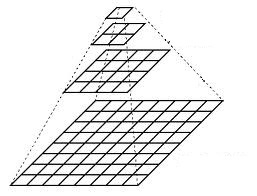
\includegraphics[width=0.90\textwidth]{imagini/Pyramids_Tutorial_Pyramid_Theory.png}
	\caption{Piramida de imagini}
	\label{fig:Pyramids_Tutorial_Pyramid_Theory}
\end{figure}

\begin{figure}[H]
	\centering
		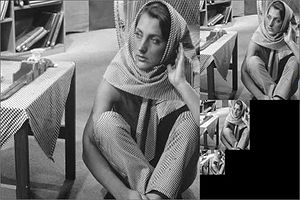
\includegraphics[width=0.90\textwidth]{imagini/300px-Example_pyramid.jpg}
	\caption{Exemplu piramida de imagini}
	\label{fig:300px-Example_pyramid}
\end{figure}


Prezentarea formarii piramidei de imagini în pseudo-cod:
\begin{mdframed}
\begin{verbatim}
sursa = citeste_imagine()
alpha = 6/5
dim_min = (100,100)
piramida = [sursa, ]
L=1
cicleaza
  D = sursa.D * 1/(alpha^L)
  daca D < dim_min
    atunci paraseste ciclul
  sfarsit daca
  nivel = scaleaza(sursa, D)
  piramida = insereaza(piramida, nivel)
  L = L + 1
sfarsit cicleaza
\end{verbatim}
\end{mdframed}

Se poate observa ca totuși acest model nu poate reprezenta toate scările posibile, find un model discret, aceasta problema poate fi ameliorata prin alegerea unui ${\alpha}$ potrivi și permițând modelului din baza de date sa reprezinte și el mici variații de scara.

O alta observație ar fi, cu cat ${\alpha}$ este mai mic, cu atât șansele sa nimerim scara corecta cresc, dar în același timp creste și consumul de memorie și durata de execuție a algoritmului. Consumul de memorie poate fi evitat dacă algoritmul se executa într-un mod recursiv, astfel eliminând menținerea explicita a unei liste de imagini în memorie.

Algoritmul fereastra glisanta se folosește pentru a obține invarianta la translație a modelului.
Aici fereastra se refera la o secțiune rectangulara a imaginii.
Fereastra va avea aceiași dimensiune ca și modelul din baza de date.
Fereastra glisanta are ca parametri ${\Delta_x, \Delta_y \geq 1}$, însemnând pasul pe axa x, respectiv pasul pe axa y.

Pseudo-cod fereastra glisanta:
\begin{mdframed}
\begin{verbatim}
dx = 8
dy = 8
I = citeste_imagine()
M = citeste_model()
pentru x de la 0 la dimx(I) - dimx(I)
  pentru y de la 0 la dimy(I) - dimy(M)
    fereastra = sectiune(I, x, y, dimx(M), dimy(M))
    proceseaza(fereastra)
  sfarsit pentru
sfarsit pentru
\end{verbatim}
\end{mdframed}

Se poate vizualiza algoritmul fereastra glisanta în figura următoare:
\begin{figure}[H]
	\centering
		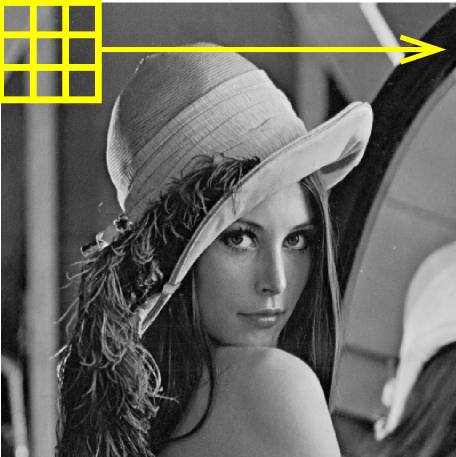
\includegraphics[width=0.70\textwidth]{imagini/AGhannoum-SlidingWindow.png}
	\caption{Fereastra glisanta}
	\label{fig:AGhannoum-SlidingWindow}
\end{figure}


Se observa ca și aici, ca și în cazul piramidei de imagini, cu cat x și y sunt mai mici cu atât creste și numărul de ferestre evaluate, ceea ce duce la un timp de execuție mai ridicat.

Complexitatea algoritmului piramida combinat cu fereastra glisanta este 
$${O((dim_x-\Delta_x)*(dim_y-\Delta_y)*n_{piramida})}$$

\pagebreak
\section{Extragerea de trăsături}

Extragerea de trăsături se ocupa cu, în cazul nostru, calcularea unei reprezentări a imaginii potrivite pentru recunoaștere.

O imagine este reprezentata ca o matrice de intensități.
Aceasta reprezentare este foarte sensibila la condițiile de iluminare, conține informații irelevante și redundante.
Se poate observa efectul iluminării în figura \ref{fig:efectul_iluminarii}.

\begin{figure}[H]
	\centering
		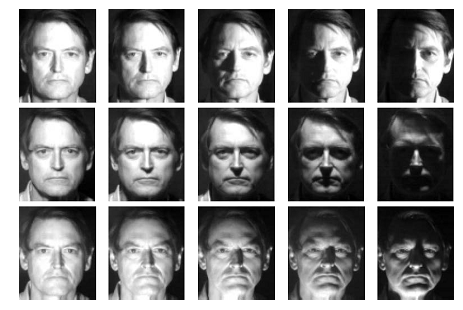
\includegraphics[width=0.90\textwidth]{imagini/efectul_iluminarii.png}
	\caption{Efectul iluminarii}
	\label{fig:efectul_iluminarii}
\end{figure}

Exista modalități de a remedia efectul iluminării, cum ar fi egalizarea histogramei(fig. \ref{fig:egalizarea_histogrameis}).
O alta modalitate ar fi sa se folosească o reprezentare pe baza de gradienți care sunt invarianți la iluminare.

\begin{figure}[H]
	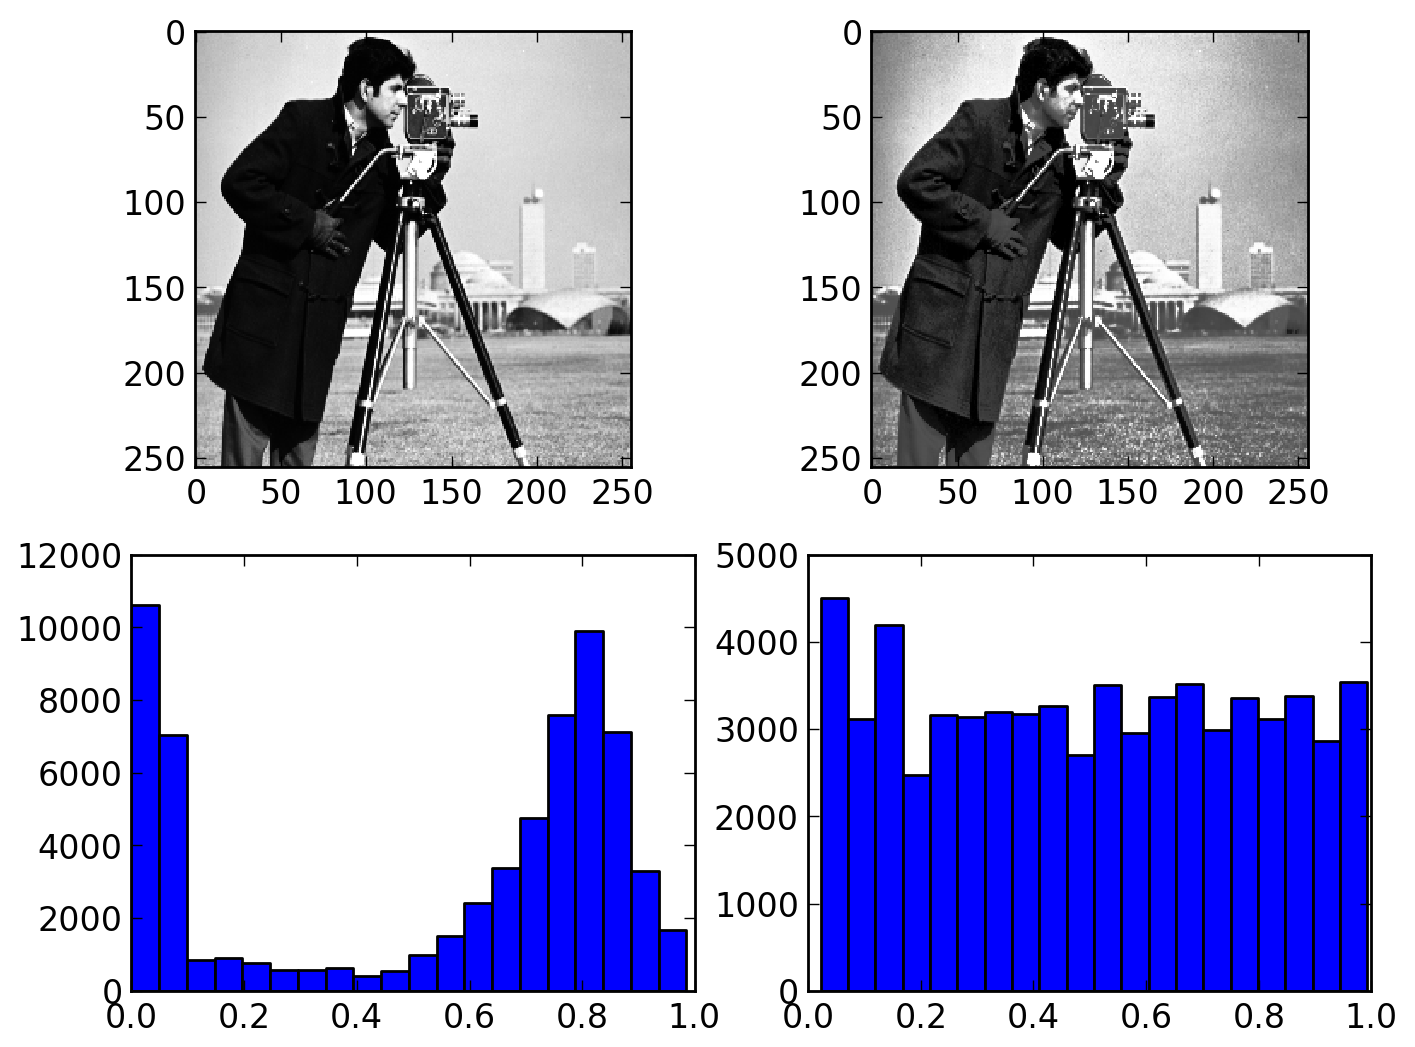
\includegraphics[width=0.90\textwidth]{imagini/HistogramEqualization-1.png}
	\caption{Egalizarea Histogramei}
	\label{fig:egalizarea_histogrameis}
\end{figure}


Efectul informațiilor irelevante și redundante poate fi ameliorat folosind tehnici de reducerea de dimensionalitate, cum ar fi analiza componentelor principale\footnote{eng. PCA, principal component analisys}(fig. \ref{fig:fig_pca_principal_component_analysis} sau transformata cosinus discreta(fig. \ref{fig:take_DCT}).

\begin{figure}[H]
	\centering
		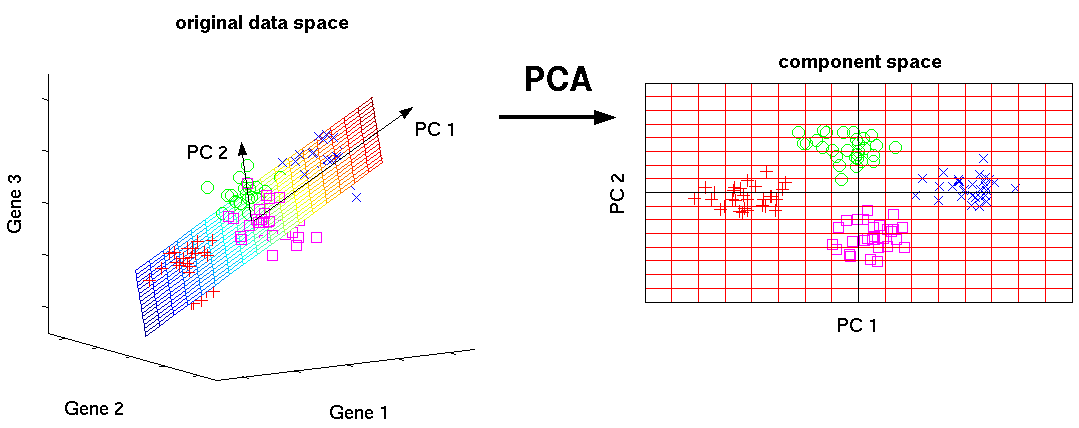
\includegraphics[width=0.90\textwidth]{imagini/fig_pca_principal_component_analysis.png}
	\caption{Analiza componentelor principale}
	\label{fig:fig_pca_principal_component_analysis}
\end{figure}

\begin{figure}[H]
	\centering
		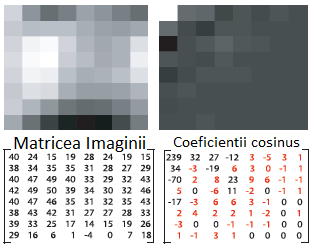
\includegraphics[width=0.90\textwidth]{imagini/take_DCT.png}
	\caption{Transformata cosinus}
	\label{fig:take_DCT}
\end{figure}



Totuși nici una dintre reprezentările menționate mai sus nu tratează problema discriminării, adică dacă doua imagini conțin același obiect atunci și reprezentările lor trebuie sa fie apropiate, iar dacă sunt imagini ale unor obiecte diferite atunci reprezentările lor sa fie distanțate.

Aici intervine ceea ce se numește ingineria trăsăturilor\footnote{eng. Feature Engineering} care, folosind cunoștințe din fizica, biologie sau chiar neurologie construiește reprezentări mult mai favorabile recunoașterii.
Câteva dinte cele mai cunoscute trăsături sunt Haar\cite{Viola01robustreal-time}, Sift\cite{Lowe99objectrecognition} și Hog\cite{Dalal05histogramsof}.

Valoare unei trăsături Haar este diferența dintre suma pixelilor din dreptunghiul negru și suma pixelilor din dreptunghiul alb, normalizata la aria celor doua.
\begin{figure}[H]
	\centering
		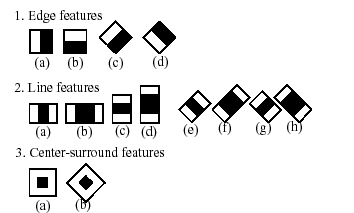
\includegraphics[width=0.90\textwidth]{imagini/haarfeatures.png}
	\caption{Trasaturi Haar}
	\label{fig:haarfeatures}
\end{figure}

Hog, sau histograma orientărilor de gradienți, se calculează divizând imaginea in zone mai mici, numite celule, apoi se calculează histograma de orientări a gradienților din aceste zone. 
Concatenarea acestor histograme reprezentând trăsătura hog.
\begin{figure}[H]
	\centering
		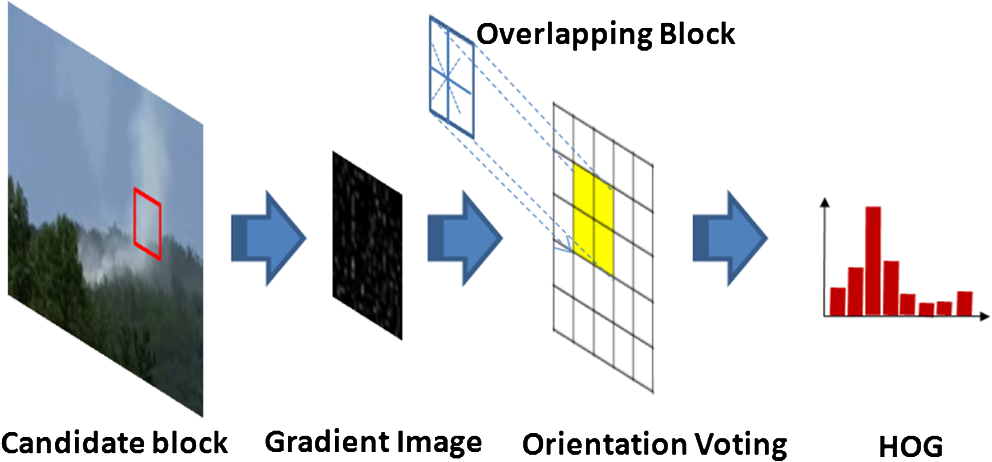
\includegraphics[width=0.90\textwidth]{imagini/OE_51_1_017208_f004.png}
	\caption{Trasaturi hog}
	\label{fig:OE_51_1_017208_f004}
\end{figure}

Descriptorul Sift este similar cu Hog, acesta find în plus și invariant la rotație.
\begin{figure}[H]
	\centering
		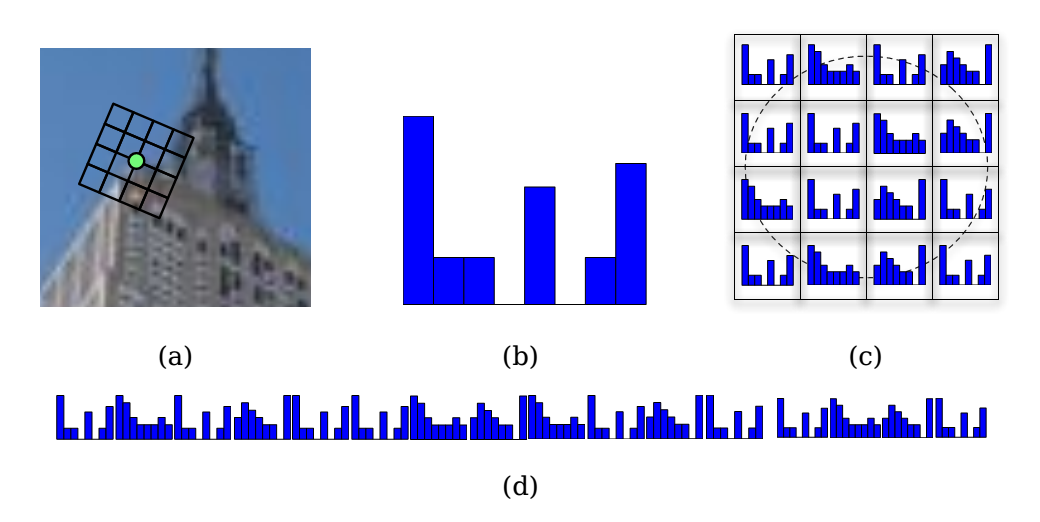
\includegraphics[width=0.90\textwidth]{imagini/sift.png}
	\caption{Descriptorul Sift}
	\label{fig:sift}
\end{figure}

Recent a apărut o noua abordare, în ceea ce privește extragerea de trăsături, aceasta folosește reprezentarea cruda a imaginii, adică matricea de intensități a pixelilor și se bazează pe algoritmul de clasificare sa extragă trăsături mai puternice, un exemplu ar fi rețeaua neurala convolutionala.\cite{lecun-98}

\pagebreak
\section{Clasificare}

Din perspectiva recunoașterii obiectelor, clasificarea se va realiza cu ajutorul unei funcții care evaluează un vector de trăsături și decide dacă este sau nu obiectul pe care încercam sa îl recunoaștem. 
Acest tip de clasificare se numește clasificare binara, findcă răspunsul nu poate lua decât doua valori.

Aceasta funcție de decizie poate fi, în cazurile cele mai simple, o funcție de prag peste o distanta euclidiana sau chiar o rețea neuronala cu sute de neuroni.

În cazul nostru aceasta funcție este rezultatul unui algoritm de învățare automata.\footnote{Machine Learning}
Învățarea automata, o ramura a inteligentei artificiale, este preocupata cu construcția și studiul sistemelor care pot învață din date.
Algoritmii de învățare automata sunt împărțiți în multe categorii, însa noi ne vom axa doar pe cei de învățare supervizata.
Se numesc algoritmi de învățare supervizata, acei algoritmi care folosesc la antrenament seturi de perechi de date ${(x,y)}$ unde ${x}$ reprezinta trăsăturile sau atributele unui exemplar, iar ${y}$ reprezinta răspunsul dorit. 
După ce a avut loc învățarea, algoritmul va fi capabil sa producă un răspuns și în cazul unor exemplare pe care nu le-a mai întâlnit, de aceea în literatura de specialitate clasificatori se mai numesc și predictori.

Scopul învățării automate, dacă privim problema din punct de vedere geometric, este acela de a găsi o un plan care sa separe cele doua clase intre ele.

\begin{figure}[h]
	\centering
		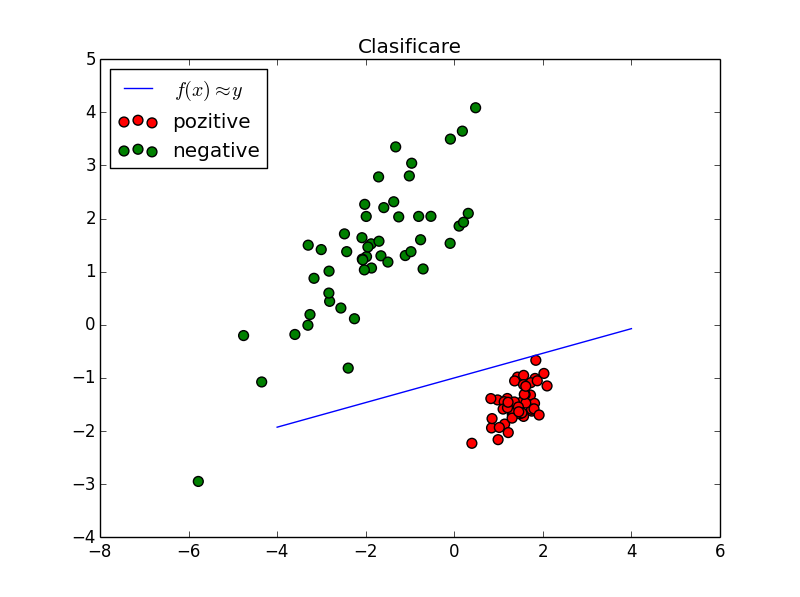
\includegraphics[width=0.90\textwidth]{imagini/fig_clasificare.png}
	\caption{Clasificare}
	\label{fig:fig_clasificare}
\end{figure}

Cel mai des întâlniți algoritmi de învățare în viziunea artificiala sunt: automatul cu vectori de suport\footnote{eng. Support Vector Machines}, rețeaua neuronala.

\pagebreak
\section{Post-procesarea rezultatelor}

O situație foarte des întâlnita în cazul algoritmilor de recunoaștere a imaginilor este ca același obiect este detectat de mai multe ori.
Aceste detecții sunt suprapuse și se datorează faptului ca modelul învățat recunoaște și obiecte cu mici translații și scalari.
Totuși, se dorește ca fiecare obiect prezent în imagine sa fie detectat doar o singura data.
Acest lucru se realizează cu ajutorul unui algoritm de grupare a detecțiilor suprapuse.

\pagebreak
\section{Algoritmul de recunoaștere}

Folosindu-ne de componentele descrise în acest capitol putem discuta despre algoritmii de recunoaștere și antrenarea lor.

Algoritmul de recunoaștere a obiectelor poate fi descris cu ajutorul pseudo-codului urmator:
\begin{mdframed}
\begin{verbatim}

detectii = lista_goale()

I = citeste_imaginea()
P = construieste_piramida(I)

pentru fiecare nivel din P
  pentru fiecare fereastra din extrage_ferestele(P)
    trasaturi = extrage_trasaturi(fereastra)
    raspuns = clasificare(trasaturi)
    daca rasuns este afirmativ atunci
      detectii = adauga(detectii, locatie(fereastra))
    sfarsit daca
  sfarsit
sfarsit

detectii = grupare_suprapuse(detectii)

\end{verbatim}
\end{mdframed}

Pentru antrenarea unui algoritm de recunoaștere a obiectelor avem nevoie de o baza de date cu doua seturi de imagini.
Un set va conține imagini decupate cu obiectul pe care dorim sa îl recunoaștem, iar al doilea va fi constituit din imagini care nu conțin obiectul.
Aceste seturi se numesc setul de exemplare pozitive, respectiv negative.
Setul de pozitive este adus la o mărime comuna prin redimensionare.
Din setul de imagini negative se vor extrage exemplare folosind scanarea în scara și spațiu de la algoritmul de recunoaștere.
Pentru ca setul de negative este de obicei foarte mare, nu este practic ca la antrenare sa se folosească toate exemplarele posibile.
Exemplarele negative se vor extrage printr-un proces iterativ.
În prima faza se extrag un număr ales de exemple negative și se antrenează clasificatorul.
Pe urma folosind clasificatorul antrenat la pasul anterior se scanează imaginile negative, fiecare exemplar negativ care a fost clasificat pozitiv se adaugă la lista de antrenare și se antrenează clasificatorul din nou.
Pasul asta se repeta de un număr de ori specificat de utilizator, ori pana când nu se mai pot extrage exemplare negative din setul de date.
Acesta se procedeu se numește bootstrapping.

\begin{mdframed}
\begin{verbatim}

P = citeste_setul_de_exemplare_positive()
N = citeste_setul_de_exemplare_negative()

X = lista()
y = lista()

X = adauga(X, P)
y = adauga(y, selecteaza_aleator(N))

Cls = antreneaza_clasificator(X,y)

iter = citeste_nr_iteratii()

pentru i = 1 pana la iter
  pentru I din N
    P = construieste_piramida(I)
    pentru fiecare nivel din P
      pentru fiecare fereastra din extrage_ferestele(P)
        xi = extrage_trasaturi(xi)
        raspuns = clasificare(Cls, xi)
        daca rasuns este 'afirmativ' atunci
          X = adauga(X, xi)
          y = adauga(y, 'negativ')
        sfarsit daca
      sfarsit
    sfarsit
  sfarsit
  
  Cls = antreneaza_clasificator(X,y)
sfarsit

\end{verbatim}
\end{mdframed}



















